\section{Reading text from Loday-Richaud}
\begin{itemize}
  \item \textbf{The paper:}
    \cite{Loday1994}
    \begin{itemize}
      \item Stokes matrices are not all germs of isotropies, only the Sokes
        germs! see 4.3.13
      \item for \textbf{Sheaf $\to$ Matrix}
        \begin{thm}[II.2.1]
          The map
          \[
            h:\prod_{\alpha\in\A}\Sto_\alpha(A_0)\to H^1(S^1;\Lambda(A_0))
          \]
          is bijective and natural.
        \end{thm}
    \end{itemize}
  \item \textbf{The book:} \cite{lodayrichaud:hal-01011050}
    \begin{itemize}
      \item multilevels, multisectors
    \end{itemize}
  \item others:
    \begin{itemize}
      \item \cite{LodayRichaud2004}
    \end{itemize}
\end{itemize}

\subsection{Determination $\tilde\theta$ of $\theta$}
\begin{center}
  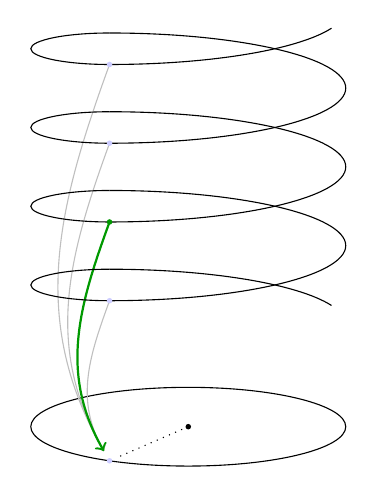
\begin{tikzpicture}[scale=1]
    \node[] (zero) at (0,0) {};
    \fill (zero) circle (1pt);
    \draw (0,-0.5) arc (270:-90:2 and 0.5);

    \node (theta) at ({cos(240) * 2},{sin(240) * 0.5}) {};
    % \node [below left of=theta,blue!40!white] {$\theta$};

    \draw[->,gray!50!white] (-1,1.6) to[out=250,in=120] (theta);
    \draw[->,gray!50!white] (-1,3.6) to[out=250,in=120] (theta);
    \draw[->,gray!50!white] (-1,4.6) to[out=250,in=120] (theta);
    \draw[->,green!60!black,thick] (-1,2.6) to[out=250,in=120] (theta);

    \draw[dotted] (0,0) -- (theta);
    \fill[blue!20!white] (theta) circle (1pt);


    \draw[] (-1,2) arc (270:200:-3 and -0.7);
    \draw[] (-1,2) arc (270:90:1 and -0.2) arc (270:90:-3 and 0.7);
    \fill[blue!20!white] (-1,1.6) circle (1pt);
    \draw[] (-1,3) arc (270:90:1 and -0.2) arc (270:90:-3 and 0.7);
    \fill[green!60!black] (-1,2.6) circle (1pt);
    \draw[] (-1,4) arc (270:90:1 and -0.2) arc (270:90:-3 and 0.7);
    \fill[blue!20!white] (-1,3.6) circle (1pt);
    \draw[] (-1,5) arc (270:90:1 and -0.2) arc (270:200:-3 and 0.7);
    \fill[blue!20!white] (-1,4.6) circle (1pt);
  \end{tikzpicture}
\end{center}

\subsection{Definition of $\Lambda_\theta(A_0)$}
$\Lambda_\theta(A_0)$ $:\Leftrightarrow{}$ sheaf of flat isotropies over $S^1$
\marginnote{p. 854f \cite{Loday1994}}
\begin{defn}
  A germ of $\Lambda_\theta(A_0)$ at $\theta_0\in S^1$ is
  \begin{itemize}
    \item an invertible Matrix $f\in\Gl_n(\cO(U))$ 
      \begin{itemize}
        \item for suitable arc $U=U(\theta_0,\epsilon,\epsilon')$
      \end{itemize}
      satisfying:
      \begin{enumerate}
        \item \emph{Flatness:}
          \[
            \underset{x\in U}{\underset{x\to0}{\lim}}f(x)=\Id
            \text{ and }
            f\underset{U}{\sim}I
          \]
        \item \emph{Isotropy of $[A_0]$: ${}^fA_0=A_0$.}
      \end{enumerate}
  \end{itemize}
\end{defn}

\begin{center}
  \begin{tikzpicture}[scale=1]
    \node[] (zero) at (0,0) {};
    \fill (zero) circle (1pt);
    \draw (0,2) arc (270:-90:0.5 and 2);

    \fill[blue!20!white] (theta) circle (1pt);

    \filldraw[fill=green!20!white
      ,draw=green!60!black
      ,thick
    ,path fading=west] (0,0)
      -- ({cos( -50 )*4},{sin( -50 )*1}) arc (-50:20:4 and 1)
      -- cycle;

    \filldraw[fill=white,draw=green!60!black] (0,4)
      -- +({cos( -50 )*0.5},{sin( -50 )*2}) arc (-50:20:0.5 and 2)
      -- cycle;

    \filldraw[fill=gray,draw=green!60!black] (0,4)
      -- ({cos( -50 )*0.5},{4 + sin( -20 )*2})
      -- ({cos( -50 )*0.5 + cos( -20 )*0.5}
        ,{4 + sin( -50 )*2 + sin( -50 )*2})
      arc (-50:20:0.5 and 2)
      -- cycle;

    \draw[blue!60!black] (zero) -- ({cos( -15 )*4},{sin( -15 )*1});

    \draw[dashed] (zero) -- (0,2);
  \end{tikzpicture}
\end{center}

\subsection{Definition of $\Sto_\alpha(A_0)$}
\begin{itemize}
  \item p. 861 in the paper
  \item p. 78 in the book
\end{itemize}
